\documentclass{article}
\usepackage{graphicx} % Required for inserting images
\usepackage[margin=1in]{geometry}
\usepackage{amsmath}
\usepackage{amsfonts}
\usepackage{listings} % to write code 
\usepackage{mathabx} % \boxslash
\usepackage{float}


\title{Tensor Factorisation for Group Detection}
\author{ Ange Kokotakis, Romain Ramez \\ \small directed by Rodrigo Cabral Farias}
\date{December 2023}

\begin{document}

\maketitle

\begin{abstract}
    The aim of this project is to detect groups of people with a given dataset of interactions in a community.
    For this purpose we will represent the dataset as a tensor and use non-negative tensor factorization to approximate
    it as a product of different matrix from which we can get information about groups in this community.
\end{abstract}

\section{Introduction}

In this project, we use datasets similar to Figure \ref{dataset} in which each line represents an interaction between
two individuals: $id1$ and $id2$ at a certain $time$.

\begin{figure}[h]
    \centering
    \includegraphics[width=0.3\textwidth]{images/tableau_données.png}
    \caption{dataset}
    \label{dataset}
\end{figure}

From this dataset we create matrices $\mathbf{X} \in \{0, 1\}^{I \times I}$ which represent interactions between people during a certain
interval of time where $I$ is equal to the number of people in the community and each coefficient is equal to :

\[
    \mathbf{X}_{i,j} = 
    \begin{cases}
        1 & \text{if there is an interaction between person $i$ and $j$ during a given interval of time} \\
        0 & \text{otherwise}
    \end{cases}
\]

And then we stack these matrices with different interval $t_k$ of time to create our tensor $\mathbf{Y} \in \{0, 1\}^{I \times I \times K}$
where K is the number of intervals of time. Finally the tensor containing the dataset has its coefficients equal to :

\[
    \mathbf{Y}_{i,j,k} = 
    \begin{cases}
        1 & \text{if there is an interaction between person $i$ and $j$ at interval of time $t_k$} \\
        0 & \text{otherwise}
    \end{cases}
\]

\section{Model}

In order to approximate this tensor we create 3 matrices :
\[
    \mathbf{U} \in \mathbb{R}_+^{I \times R}, \,
    \mathbf{V} \in \mathbb{R}_+^{I \times R}, \,
    \mathbf{W} \in \mathbb{R}_+^{K \times R}
\]

where :
\begin{itemize}
    \item[]
    \begin{itemize}
        \item $I$ is the number of individuals in the community,
        \item $K$ is the number of interval of time,
        \item $R$ is the number of groups in the community (we choose one randomly at first we will see later how to choose it correctly).
    \end{itemize}
\end{itemize}

The $U$ and $V$ matrices represent the membership level of a person to a certain group
and $W$ represents in which interval of time a group has been active.

% \[
%     L(U, V, W)=\|Y-[U, V, W]\|_{F}^2 +\lambda \|U-V\|_{F}^2
% \]

%\section{Multiplication Update Algorithm (MU)}

% \begin{lstlisting}[language=Python]
    % code
% \end{lstlisting}

We define $\mathbf{S} \in \mathbb{R}_+^{I \times I \times K}$ as :

\[
    \mathbf{S}_{i,j,k} = \sum_{r = 1}^R \mathbf{U}_{i,r}\mathbf{V}_{j,r}\mathbf{W}_{k, r}
\]

The result of the product $\mathbf{U}_{i,r}\mathbf{V}_{j,r}\mathbf{W}_{k, r}$ is called the outer product noted $\mathbf{U}_r \circ \mathbf{V}_r \circ \mathbf{W}_r$ which can be seen as :

\begin{figure}[h]
    \centering
    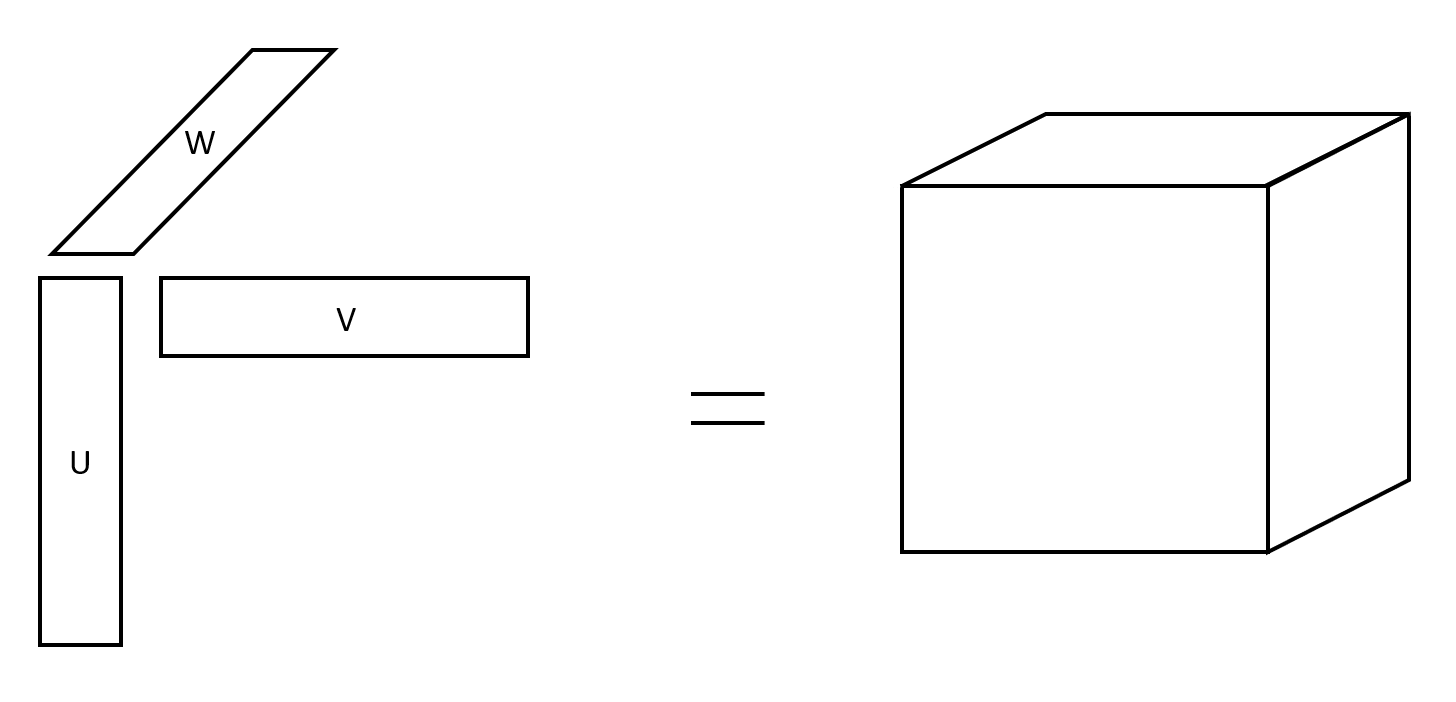
\includegraphics[width=0.5\textwidth]{images/outer_product.png}
\end{figure}


Finally S is define as : 
\[
    \mathbf{S} = \sum_{r = 1}^R \mathbf{U}_r \circ \mathbf{V}_r \circ \mathbf{W}_r
\]

In order to approximate Y with S we define a cost fonction $L(\mathbf{U}, \mathbf{V}, \mathbf{W})=\|\mathbf{Y}-\mathbf{S}\|_{F}^2$ where $\|.\|_F$ represents the Frobenius norm,
moreover because U and V are representing the same thing we want these matrices to be similar so we add to L another term $\lambda\|\mathbf{U}-\mathbf{V}\|_{F}^2$.
 Finally $L$ is defined by :

\[
    L(\mathbf{U}, \mathbf{V}, \mathbf{W})=\|\mathbf{Y}-\mathbf{S}\|_{F}^2 +\lambda \|\mathbf{U}-\mathbf{V}\|_{F}^2, \lambda \in \mathbb{R}_+
\]

$L$ can be rewritten by using unfolded forms of $\mathbf{Y}$ i.e. by transforming it in a matrix with all the layers of $\mathbf{Y}$
arranged in different ways and by using Khatri-Rao product $\odot$ :

\begin{align*}
L(\mathbf{U}, \mathbf{V}, \mathbf{W}) &= \|\mathbf{Y}^{(1)}-\mathbf{U}(\mathbf{W}\odot \mathbf{V})^{T}\|_{F}^2 +\lambda \|\mathbf{U}-\mathbf{V}\|_{F}^2 \\
                &= \|\mathbf{Y}^{(2)}-\mathbf{V}(\mathbf{W}\odot \mathbf{U})^{T}\|_{F}^2 +\lambda \|\mathbf{U}-\mathbf{V}\|_{F}^2\\
                &= \|\mathbf{Y}^{(3)}-\mathbf{W}(\mathbf{V}\odot \mathbf{U})^{T}\|_{F}^2 +\lambda \|\mathbf{U}-\mathbf{V}\|_{F}^2
\end{align*}

To minimize this function we will use two
different method : the multiplicative update algorithm (MU) and the hierarchical alternating least square (HALS) and these forms of
$L$ will be very useful.

\section{Multiplicative Update}
The principle of this algorithm is to alternatively minimize $L$ with respect to each of its components by
using a version of gradient algorithm.

At each iteration we calculate :

\[\nabla L = \begin{bmatrix}
                \nabla_{\mathbf{U}} L\\
                \nabla_{\mathbf{V}} L \\
                \nabla_{\mathbf{W}} L 
            \end{bmatrix} = \begin{bmatrix}
                                [\nabla_{\mathbf{U}} L]^{+}-[\nabla_{\mathbf{U}} L]^{-}\\
                                [\nabla_{\mathbf{V}} L]^{+}-[\nabla_{\mathbf{V}} L]^{-} \\
                                [\nabla_{\mathbf{W}} L]^{+}-[\nabla_{\mathbf{W}} L]^{-} 
                            \end{bmatrix}
\]

Where all the $[.]^{+}, [.]^{-}$ are positive

Then we update $\mathbf{U}, \mathbf{V}$ and $\mathbf{W}$ :
\begin{align*}
    &\mathbf{U}_{k} = \mathbf{U}_{k-1}\boxdot ([\nabla_{\mathbf{U}} L]^{+}\boxslash[\nabla_{\mathbf{U}} L]^{-}) \\
    &\mathbf{V}_{k} = \mathbf{V}_{k-1}\boxdot ([\nabla_{\mathbf{V}} L]^{+}\boxslash[\nabla_{\mathbf{V}} L]^{-}) \\
    &\mathbf{W}_{k} = \mathbf{W}_{k-1}\boxdot ([\nabla_{\mathbf{W}} L]^{+}\boxslash[\nabla_{\mathbf{W}} L]^{-})
\end{align*}
Where $\boxdot$ and $\boxslash$ are the Hadamard product and division respectively. To avoid division by zero, we replace all the zero coefficient by an epsilon strictly positive.




\section{Hierarchical Alternating Least Square}
This algorithm minimize $L$ with respect to one column of $\mathbf{U}$, $\mathbf{V}$ or $\mathbf{W}$ at a time, all the other column are fixed to their previous approximation
for instance with the column $\mathbf{U}_{r'}$ :

\begin{align*}
      &\,\, L = \|\mathbf{Y}-\mathbf{S}\|_{F}^2 +\lambda \|\mathbf{U}-\mathbf{V}\|_{F}^2 \\
      &= \sum_{ijk}(\mathbf{Y}_{ijk}-\sum_{r \ne r'}(\mathbf{U}_{ir}\mathbf{V}_{jr}\mathbf{W}_{kr})-\mathbf{U}_{ir'}\mathbf{V}_{jr'}\mathbf{W}_{kr'})^{2}+\lambda\sum_{i}\sum_{r \ne r'}(\mathbf{U}_{ir}-\mathbf{V}_{ir})^{2}+\lambda\sum_{i}(\mathbf{U}_{ir'}-\mathbf{V}_{ir'})^{2}\\
      &= \sum_i \mathbf{U}_{ir'}^2(\lambda I + \sum_{jk}(\mathbf{W}_{kr'}\mathbf{V}_{kr'})^2) - 2 \mathbf{U}_{ir'}(\lambda \mathbf{V}_{ir'} + \sum_{jk}\mathbf{W}_{kr'}\mathbf{V}_{kr'}(\mathbf{Y}_{ijk}-\sum_{r \ne r'}(\mathbf{U}_{ir}\mathbf{V}_{jr}\mathbf{W}_{kr}))) + C , \text{C independent of $\mathbf{U}_{ir'}$ }\\
      &\text{So $L$ is minimum with respect to $\mathbf{U}_{ir'}$ if } \mathbf{U}_{ir'} = \frac{\lambda \mathbf{V}_{ir'} + \sum_{jk}\mathbf{W}_{kr'}\mathbf{V}_{kr'}(\mathbf{Y}_{ijk}-\sum_{r \ne r'}(\mathbf{U}_{ir}\mathbf{V}_{jr}\mathbf{W}_{kr}))}{\lambda I + \sum_{jkr'}(\mathbf{W}_{kr'}\mathbf{V}_{kr'})^2}
\end{align*}

We can generalize this result to an entire column : $\mathbf{U}_{:,r'} = \frac{\lambda \mathbf{V}_{:,r'} + \sum_{jk}\mathbf{W}_{kr'}\mathbf{V}_{kr'}(\mathbf{Y}_{:,jk}-\sum_{r \ne r'}(\mathbf{U}_{:,r}\mathbf{V}_{jr}\mathbf{W}_{kr}))}{\lambda I + \sum_{jkr'}(\mathbf{W}_{kr'}\mathbf{V}_{kr'})^2}$,
we can find the two other update by symetry for $\mathbf{V}$ and by doing the same calcul for $\mathbf{W}$.\\

At each iteration we update $\mathbf{U}_{r'}$, $\mathbf{V}_{r'}$, $\mathbf{W}_{r'}$,  then we increment $r'$ until we reach our convergence criterion or our maximum number of iteration.

\section{Comparison of MU and HALS convergence}

We note that HALS converge fa   ster than MU.

\begin{figure}[H]
    \centering
    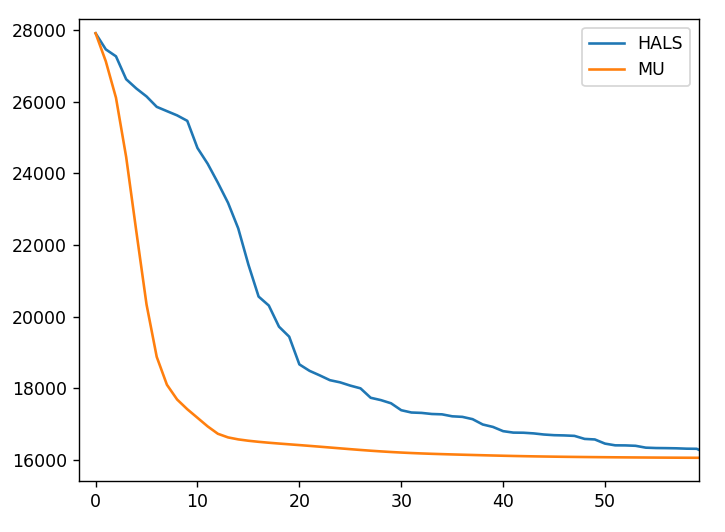
\includegraphics[width=0.5\textwidth]{images/comparison_HALS_MU.png}
    \caption{comparison between MU and HALS convergence}
\end{figure}



\section{Interpretation of our results}

In this section we use a database composed of interaction between students and teachers in a school during 2 days, this databse furnished
metadata which indicate in which class students are. We represent it as the scheme below where two people in the same class have the same color, teachers ar in black,
the distance between two individuals is randomly chosen and have no meaning in this representation :

\begin{figure}[h]
    \centering
    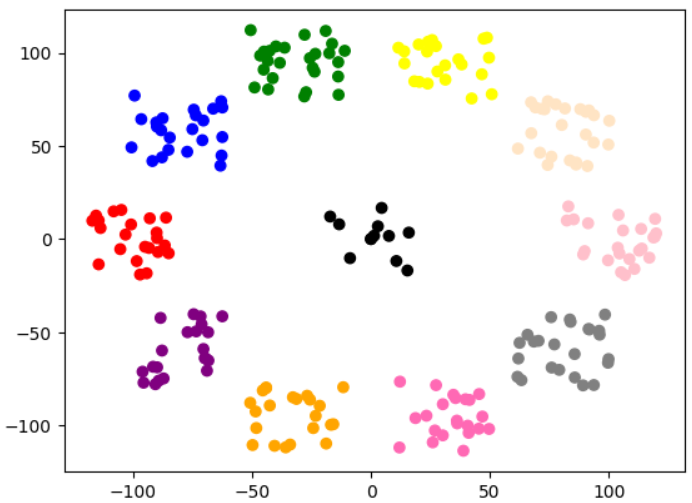
\includegraphics[width=0.5\textwidth]{images/original_class.png}
    \caption{original classes}
\end{figure}

\subsection{A first approximation}
Using $\mathbf{U}$ (and $\mathbf{V}$) we create the same representation by choosing the maximum in each line of U to determine the group of a person in the school,
we naively chose R = 11 because we can see 11 groups on the scheme above, it give us this in the best case:

\begin{figure}[h]
    \centering
    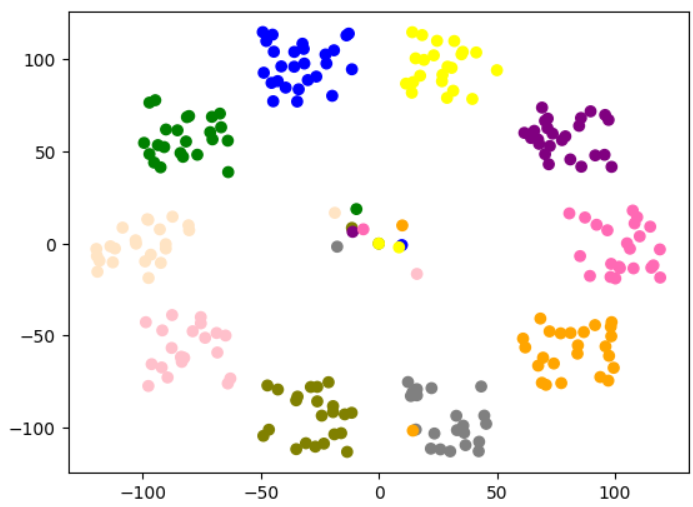
\includegraphics[width=0.5\textwidth]{images/naive_approach_r=11_t=18000.png}
    \caption{estimation with R = 11, timestep = 18000$s$}
\end{figure}

As we can see, the group of teachers is not well approximate. It can be easily explained by the fact that they have way more 
interactions with students over a day than with other professor. By checking the original database, interactions between two teachers 
represents less than 7.5\% of the total numbers of interactions between a professor and someone else. 
So teachers will finally be part of classes group and cant be detected by this model.\\

\subsection{Impact of initial conditions}
By doing this first factorization we noticed that, with these parameters, the approximation is not every time the same, 
no matter the number of iteration we do. The model is sensitive to the initial $\mathbf{U}$, $\mathbf{V}$ and $\mathbf{W}$ that we
choose randomly at the intialisation. We have mainly these 3 cases :

\begin{figure}[h]
    \centering
    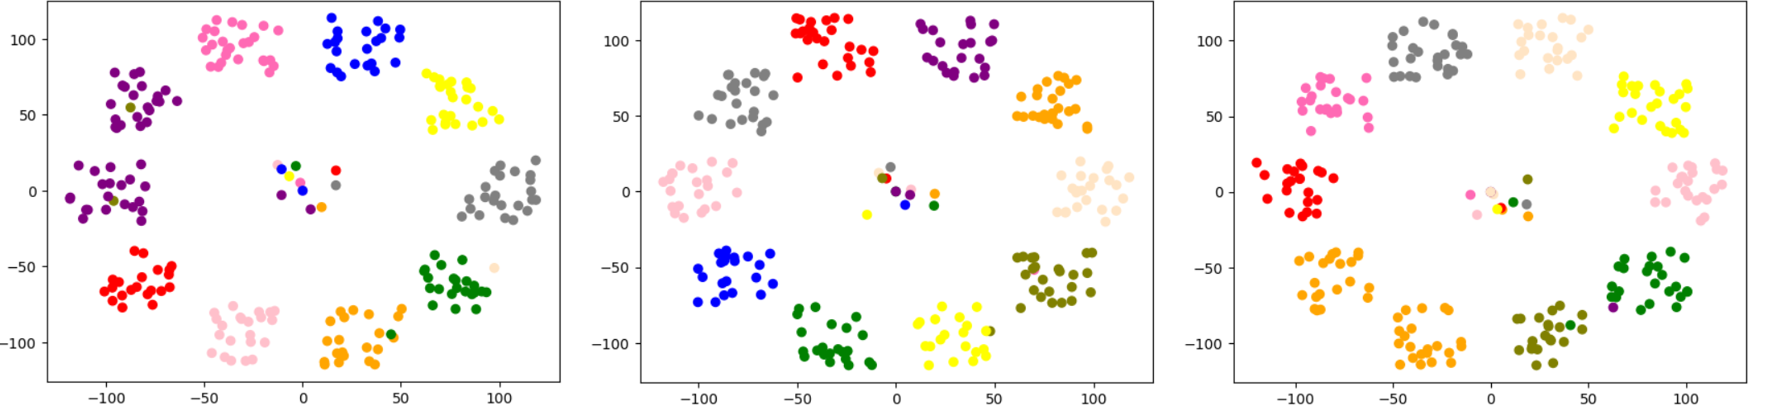
\includegraphics[width=1\textwidth]{images/3cases_of_convergence.png}
    \caption{3 differents estimations with R = 11, timestep = 18000$s$}
\end{figure}

In these 3 cases the value of L are nearly the same, we deduce from these estimations that the function L is not convexe, so the model can converge 
towards different solutions depending of the initial $\mathbf{U}$, $\mathbf{V}$ and $\mathbf{W}$.























Now that we have code the MU factorization, we can compare our results with the exact solution. 
For that, we will use several $R$ for several interval of time $t_{k}$ and change the number of iteration and see what happened. \\

\begin{figure}[h]
    \centering
    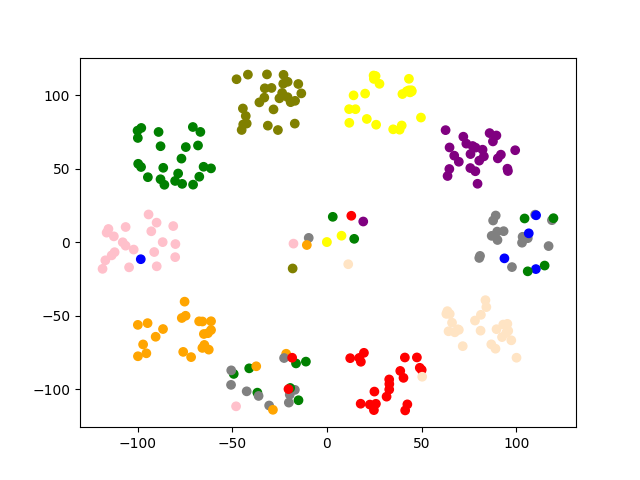
\includegraphics[width=0.5\textwidth]{images/MU50_R10_t3600.png}
    \caption{MU with $R$= 10, $t_{k}$= 3600 and $Nb_it$=50}
\end{figure}

\begin{figure}[h]
    \centering
    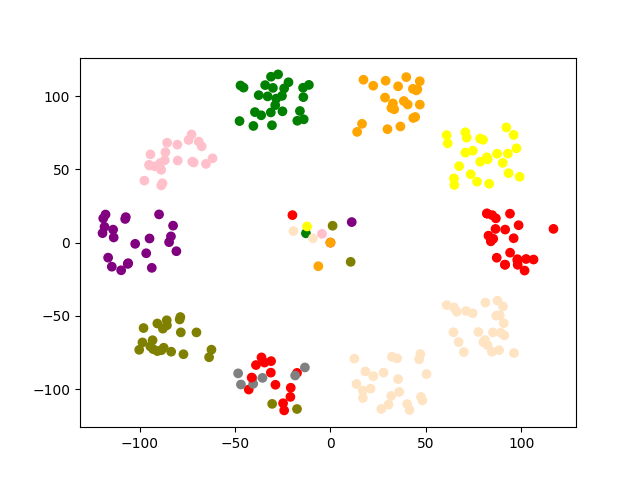
\includegraphics[width=0.5\textwidth]{images/MU150_R10_t3600.png}
    \caption{MU with $R$= 10, $t_{k}$= 3600 and $Nb_it$=150}
\end{figure}

\begin{figure}[h]
    \centering
    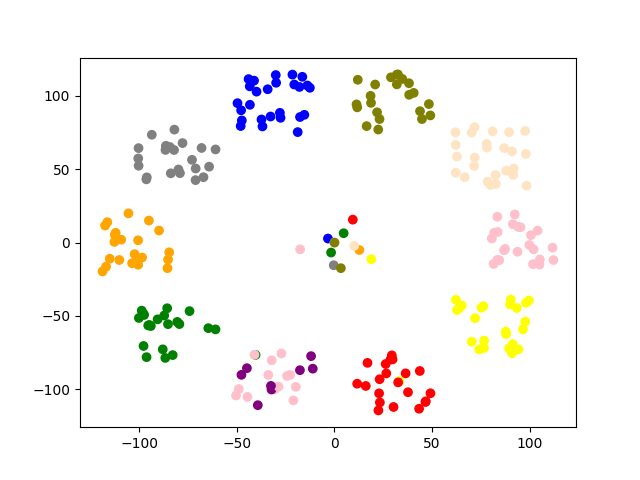
\includegraphics[width=0.5\textwidth]{images/MU500_R10_t3600.png}
    \caption{MU with $R$ = 10, $t_{k}$ = 3600 and $Nb_it$ =500}
\end{figure}

In this three first pictures, we can see the evolution of our model when we change the number of iteration.\\

In the first one, with $Nb_it$=50, we have a lot of person in the wrong group. We can count that ten persons are in another group and there's a full group made of people from others group. This model is clearly not that good.\\

It the second one, there's few people in the wrong group by still a group made by people from two other, and this time we can also see that there's two group in the same color, meaning that, in the model, the two groups are the same group. Finally, the result is better but we still have to improve this.\\

The third one is really better. Almost everyone is in his group, except the same group that is made of 2 groups, but this time we can see that there's more people from the "purple one", meaning that the group belong to them and so we can conclude that the "pinks" and the "purples" have a lot of contact with each other.\\

We can see that more the number of iteration is, more the result is close to the exact scheme. Showing the importance of this parameter.\\

\begin{figure}[h]
    \centering
    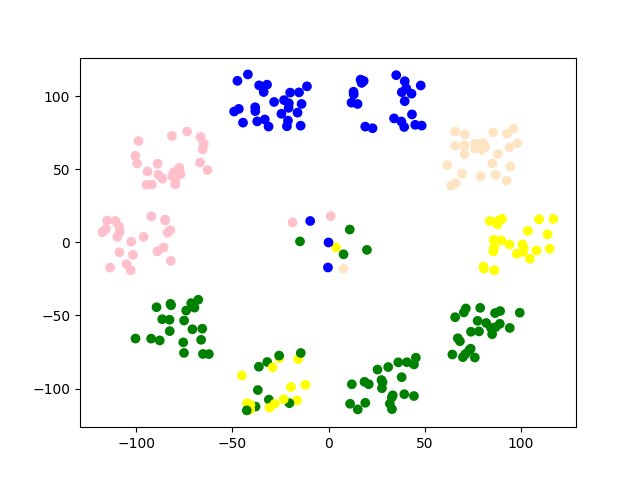
\includegraphics[width=0.5\textwidth]{images/MU500_R5_t3600.png}
    \caption{MU with $R$= 5, $t_{k}$= 3600 and $Nb_it$=500}
\end{figure}

\begin{figure}[h]
    \centering
    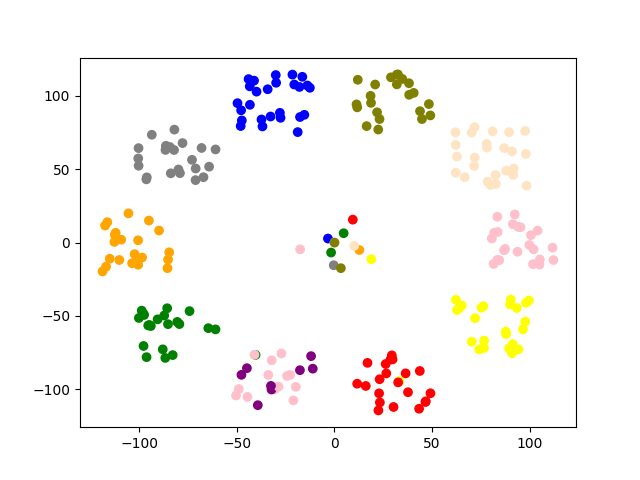
\includegraphics[width=0.5\textwidth]{images/MU500_R10_t3600.png}
    \caption{MU with $R$= 10, $t_{k}$= 3600 and $Nb_it$=500}
\end{figure}

\begin{figure}[h]
    \centering
    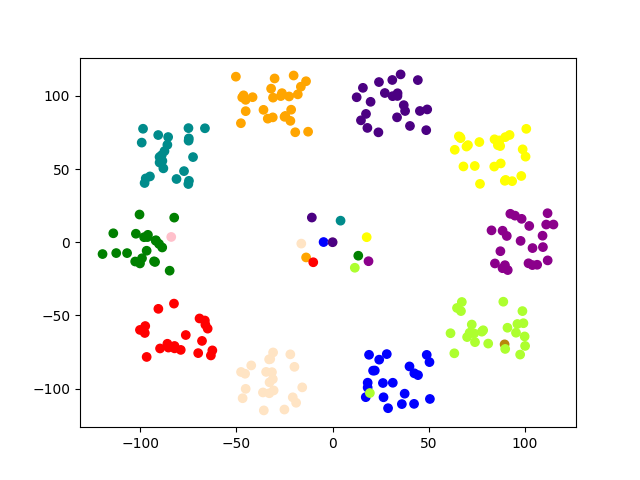
\includegraphics[width=0.5\textwidth]{images/MU500_R15_t3600.png}
    \caption{MU with $R$= 15, $t_{k}$= 3600 and $Nb_it$=500}
\end{figure}

In this three pictures, we will the how the parameter $R$ can change the result of our model.\\

In the picture 5, we have $R=5$, which means that we try to put a larger number of group in only 5 groups. That's why we have lots of group in the same color. That's bad but the fact that we have five "well" separated show that the model if still efficient. We can see that all the people from each group are still together in one of the five "big" groups.\\

In the picture 6, the result is way better. We can see ten distinct groups and almost everyone in his group. In fact, ten is the real number of group in this case. Which means ten is the minimal number for R where we can see all the group well separated.

In the last picture, we still have ten separated groups but this time the separation is better. We have only three person in the wrong group over 242 persons. We can conclude on the efficiency of the model !\\

Finally, we can see that's we have a minimum for R, which is the real number of group but passed this number, we can grown it however we want and it will always increase the model.

\begin{figure}[h]
    \centering
    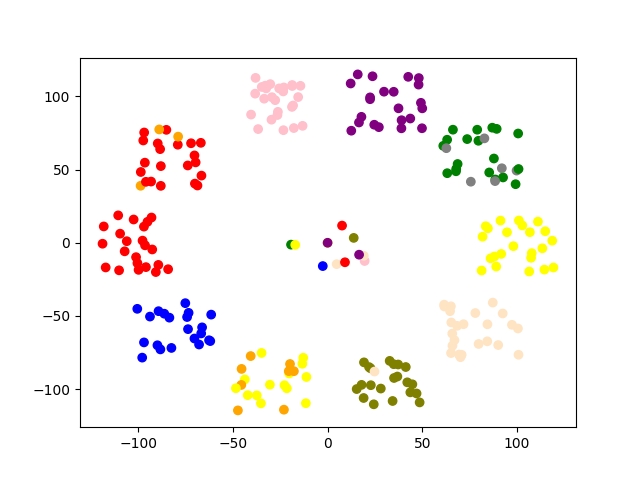
\includegraphics[width=0.5\textwidth]{images/MU500_R10_t900.png}
    \caption{MU with $R$= 10, $t_{k}$= 900 and $Nb_it$=500}

\end{figure}

\begin{figure}[h]
    \centering
    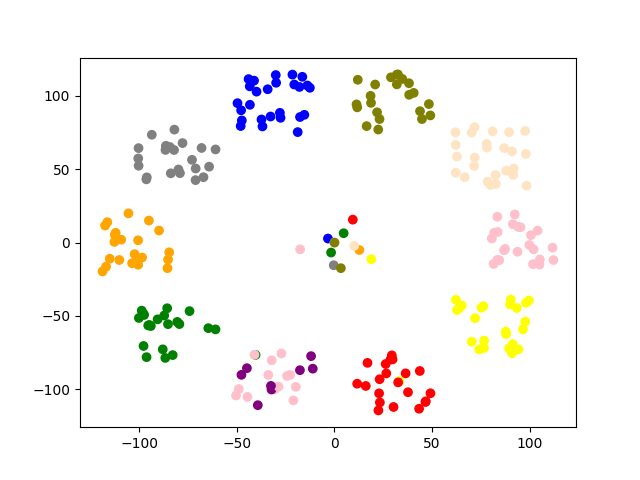
\includegraphics[width=0.5\textwidth]{images/MU500_R10_t3600.png}
    \caption{MU with $R$= 10, $t_{k}$= 3600 and $Nb_it$=500}

\end{figure}

\begin{figure}[h]
    \centering
    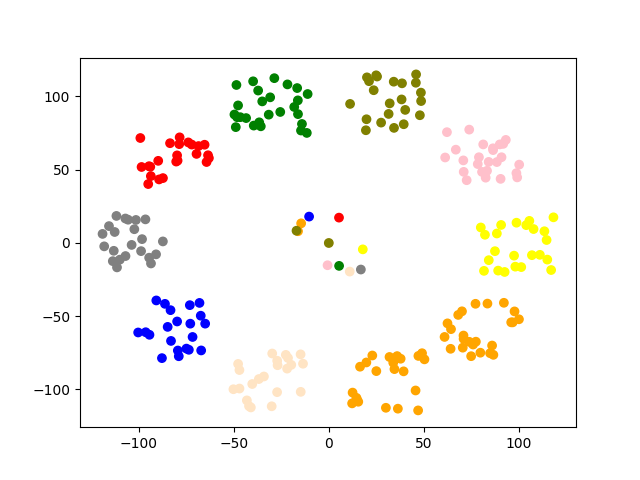
\includegraphics[width=0.5\textwidth]{images/MU500_R10_t18000.png}
    \caption{MU with $R$= 10, $t_{k}$= 18000 and $Nb_it$=500}

\end{figure}

Now, we have change the interval of time $t_{k}$.\\


    


\end{document}
%mettre en gras les matrices en gras voir mathbf